\cleardoublepage
\thispagestyle{empty}
%\thisfancypage{\setlength{\fboxsep}{5pt}\doublebox}{}
%\setlength\intextsep{0mm}
\noindent

\includegraphics[width=0.45\textwidth]{IMG/TOP/logoVSCHT_zakl_CB.png} \\
\vspace{10mm}
\\
{\Large \textbf{Fakulta  chemicko-inženýrská}
\\ [5mm]
Ústav počítačové a řídicí techniky}

\vspace{30mm}


\begin{spacing}{0.9}
\Huge\noindent POUŽITÍ ADAPTIVNÍCH SYSTÉMŮ PŘI ANALÝZE DAT\\ 
\end{spacing}
\vspace{20mm}

\noindent
{\Large \textbf{DISERTAČNÍ PRÁCE}} 

\vspace{10mm}

\begin{table}[!h]
\begin{tabular}{  l l |l  l }
\hspace{-0.5em}AUTOR & \hspace{0mm} & & {\Large \textbf{Ing. Jan Vrba}} \\ [5mm]
\hspace{-0.5em}ŠKOLITEL &  &  & \textbf{\large doc. Ing. Jan Mareš, Ph.D.}\\ [5mm]
\hspace{-0.5em}ŠKOLITEL  SPECIALISTA             &     &   & {\textbf{\large doc. Ing. Pavel Hrnčiřík, Ph.D. }} \\ [5mm]
\hspace{-0.5em}STUDIJNÍ PROGRAM &  &  & {\large Chemické a procesní inženýrství (čtyřleté)} \\ [5mm]
\hspace{-0.5em}STUDIJNÍ OBOR    & &   & {\large Technická kybernetika}\\ [5mm]
\hspace{-0.5em}ROK          &       &   & \textbf{2020} 
\end{tabular}


\end{table}

%===============================English============================
%=================================CZ===============================
\cleardoublepage
\thispagestyle{empty}
%=================================CZ================================
%============================English============================
\thispagestyle{empty}
\noindent

\includegraphics[width=0.45\textwidth]{IMG/TOP/logoUCT_basic_CB.png} \\
\vspace{10mm}
\\
{\Large \textbf{Faculty of Chemical Engineering}
\\ [5mm]
Department of Computing and Control Engineering}

\vspace{30mm}

\begin{spacing}{0.9}
\Huge\noindent ADAPTIVE SYSTEMS IN DATA \\ANALYSIS\\
\end{spacing}

\vspace{20mm}

\noindent
{\Large \textbf{DISSERTATION}} 

\vspace{10mm}

\begin{table}[!h]
\begin{tabular}{  l l |l  l }
\hspace{-0.5em}AUTHOR & \hspace{0mm} & & {\Large \textbf{Ing. Jan Vrba}} \\ [5mm]
\hspace{-0.5em}SUPERVISOR &  &  & \textbf{\large doc. Ing. Jan Mareš, Ph.D.}\\ [5mm]
\hspace{-0.5em}SUPERVISOR SPECIALIST    &     &   & {\textbf{\large doc. Ing. Pavel Hrnčiřík, Ph.D.}} \\ [5mm]
\hspace{-0.5em}STUDY PROGRAMME &  &  & {\large Chemical and Process Engineering} \\ [5mm]
\hspace{-0.5em}FIELD OF STUDY & &   & {\large Technical Cybernetics}\\ [5mm]
\hspace{-0.5em}YEAR          &       &   & \textbf{2020}
\end{tabular}


\end{table}

%%====================================================Declaration=====================
%\newpage
%\thispagestyle{empty}
%\vphantom{a}
%\vspace{13cm}
%\begin{figure}[H]
%\pdfimageresolution=133 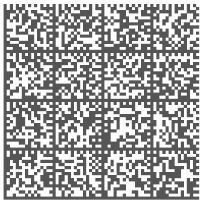
\includegraphics{IMG/TOP/QR.png}
%\end{figure}
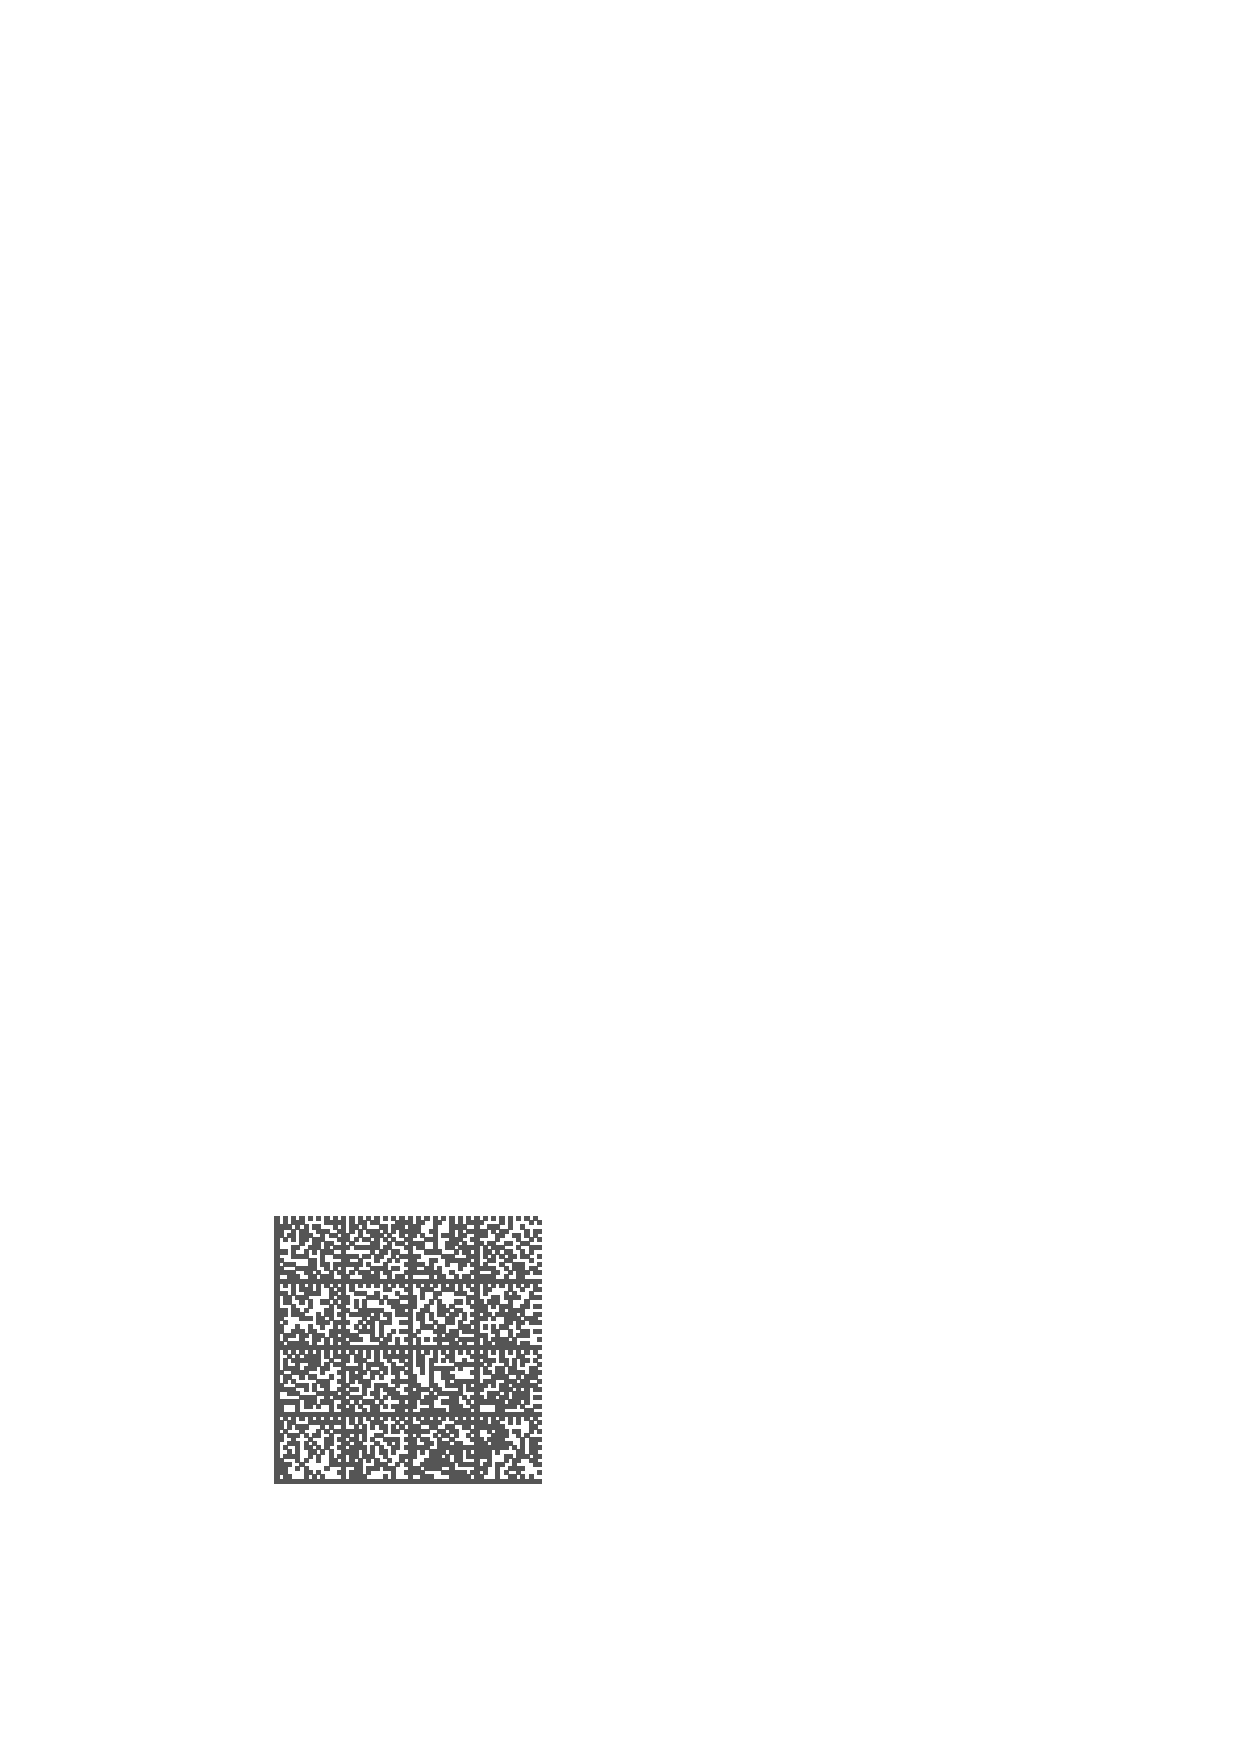
\includepdf[pages=1]{vstupni_listy-pages-4.pdf}
%%====================================================Declaration=====================
\clearpage
\thispagestyle{empty} 
 \vspace*{1cm}
 \noindent 
 Tato disertační práce byla vypracována na Ústavu počítačové a řídicí techniky
v období září 2016 -- říjen 2020. \\ [30mm]
Prohlašuji, že jsem tuto práci vypracoval samostatně. Veškeré literární prameny
a informace, které jsem v práci využil, jsou uvedeny v seznamu použité literatury. \\ [8mm]
Byl jsem seznámen s tím, že na moji práci se vztahují práva a povinnosti vyplývající
ze zákona č. 121/2000 Sb., o právu autorském, o právech souvisejících s právem
autorským a o změně některých zákonů (autorský zákon). Zejména se jedná
o skutečnost, že Vysoká škola chemicko-technologická v Praze, popř. jiné vzdělávací
zařízení, ve kterém jsem svou práci vypracoval, má právo na uzavření licenční
smlouvy o užití této práce jako školního díla podle § 60 odst. 1 autorského zákona.
Pokud bych v budoucnu poskytl licenci o užití práce jinému subjektu, je Vysoká
škola chemicko-technologická v Praze, popř. jiné vzdělávací zařízení, ve kterém
jsem svou práci vypracoval, oprávněna ode mne požadovat přiměřený příspěvek
na úhradu nákladů, které na vytvoření díla vynaložil a to podle okolností až do
jejich skutečné výše. \\ [8mm]
\noindent
Souhlasím se zveřejněním své práce podle zákona č. 111/1998 Sb., o vysokých
školách, ve znění pozdějších předpisů. \\ [30mm]


\noindent\begin{tabular}{@{}p{2.5in}p{3.in}@{}}
\hspace{1cm} V Praze dne                      &\hspace{2cm} \dotfill\\
             & \multicolumn{1}{c}{\hphantom{hhhhHHHHH}Ing. Jan Vrba}\\
\end{tabular} 

 
\cleardoublepage
\thispagestyle{empty}

 \vspace*{\fill}
 \noindent {\bf \large Poděkování} \\ [5mm]
Děkuji vedoucímu mé dizertační práce doc. Ing. Janu Marešovi, Ph.D. za všestrannou pomoc, podporu a trpělivost. Děkuji doc. Ing. Ivo Bukovskému, Ph.D.  za otevření dveří do světa detekce novosti. Rád bych poděkoval také Matouši Cejnkovi za inspiraci, blahodárné diskuze a spolupráci nejen na bitevním poli světa H\&G. Děkuji všem zaměstnancům Ústavu počítačové a řídicí techniky na VŠCHT. V neposlední řadě bych chtěl poděkovat také všem přátelům, kteří mi pomohli udržet zdravou životní rovnováhu. Zvláštní poděkování patří  mým rodičům a sestře Radaně za podporu během mého dlouhého studia. Děkuji také Otovi, který mi přinesl tolik štěstí a radosti. Nejvíce děkuji mé Kazumi za podporu, trpělivost, obětavost a za vytvoření ideálních podmínek, ve kterých jsem mohl práci psát. Děkuji.

 





%-------------------------------Abstract CZ ---------------------------------------------
\cleardoublepage
\thispagestyle{empty}
%-------------------------------Abstract CZ ---------------------------------------------

\noindent {\bf \large Souhrn} \\ [5mm]
Dizertační práce se zabývá použitím adaptivních systémů v oblasti detekce novosti. Využití adaptivních systémů pro detekci novosti v datech se stalo v posledních letech slibným směrem výzkumu. V rámci této práce je navržen nový algoritmus, využívající adaptivní systémy, pojmenovaný jako Extreme Seeking Entropy. Tento algoritmus je založen na vyhodnocování přírůstku adaptivních parametrů systémů pomocí zobecněného Paretova rozdělení. Navržený algoritmus byl otestován na celé řadě typů syntetických dat, která reprezentují různé druhy novosti. Pro detekci změny trendu a skokové změny generátoru signálu pak bylo provedeno i vyhodnocení úspěšnosti detekce. Dále byla provedena experimentální studie zabývající se časovou náročností výpočtu algoritmu, vyhodnocena ROC křivka pro detekci změny trendu a provedena studie detekce epilepsie v záznamu EEG myši.\\ [5mm]
\noindent {\bf \large Klíčová slova}  \\ [5mm] \noindent {\it adaptivní systémy, detekce novosti, časové řady, extreme seeking entropy}


\cleardoublepage
\thispagestyle{empty}


%----------------------------------------------------Abstract  English--------------------------------------------------
\cleardoublepage
\thispagestyle{empty}

\noindent {\bf \large Summary} \\ [5mm] 
The dissertation deals with the use of adaptive systems in the field of novelty detection. The use of adaptive systems for detecting novelty in data has become a promising direction of research in recent years. In this work, a new algorithm was designed using adaptive systems, called Extreme Seeking Entropy. This algorithm is based on evaluating the increment of adaptive parameters of systems using a generalized Pareto distribution. The proposed algorithm has been tested on a number of types of synthetic data that represent different types of novelty. To detect a change in the trend and a step-change in the signal generator, an evaluation of the detection success was performed. Furthermore, an experimental study was performed dealing with the time consumption of the algorithm, the ROC curve was evaluated to detect a change in the trend, and a study was performed to detect epilepsy in the EEG mouse record.
\\ [5mm]



\noindent {\bf \large Keywords}  \\ [5mm]
{\it adaptive systems, novelty detection, time series, extreme seeking entropy}




%%v~v~v~v~v~v~v~v~v~v~v~v~v~v~v~v~v~v~v~v~v~v~v~v~v~v~v~v~v
%\thispagestyle{empty}
%%v~v~v~v~v~v~v~v~v~v~v~v~v~v~v~v~v~v~v~v~v~v~v~v~v~v~v~v~v
\cleardoublepage
\tableofcontents
\thispagestyle{empty}
%\addtocontents{toc}{~\hfill\textbf{Page}\par}
%\addcontentsline{toc}{chapter}{Contents}
%%v~v~v~v~v~v~v~v~v~v~v~v~v~v~v~v~v~v~v~v~v~v~v~v~v~v~v~v~v

%\newpage
%\setcounter{page}{1}

% Seznam zkratek
\cleardoublepage
\thispagestyle{empty}

\chapter*{Seznam použitých zkratek}
\begin{tabular}{ll}
AISLE					& approximate individual sample learning entropy \\
AUROC					& area under the receiver operating characteristics\\
ELBND                   & error and learning based novelty detection      \\
ESE                     & extreme seeking entropy                         \\
FIR						& finite impulse response \\
GEV                     & generalized extreme value                       \\
GMM						& Gaussian Mixture Model \\
GNGD                    & generalized normalized gradient descend         \\
GPD						& generalized Paredo distribution \\
HMM						& hidden Markov model \\
HONU					& higher order neural unit \\
IIR						& infinite impulse response \\
LE                      & learning entropy                              \\
LNU                     & linear neural unit                              \\
LMS						& least mean squares							\\
MOM						& method of moments \\
NLMS                    & normalized least mean squares                   \\
PCA						& principal component analysis \\
POT                     & peak-over-threshold                             \\
QNU                     & quadratic neural unit                           \\
RLS                     & recursive least squares                         \\
ROC						& receiver operating characteristics \\
SNR                     & signal-to-noise ratio                           \\
SM-NLMS                 & set-membership normalized least mean squares \\
SVM						& support vector machine \\



\end{tabular}

% Seznam zkratek
\cleardoublepage
\thispagestyle{empty}

\chapter*{Seznam symbolů}
\begin{tabular}{ll}
$\mathbb{N}$    & množina přirozených čísel                        \\
$\mathbb{R}$    & množina reálných čísel                          \\
$k$             & diskrétní časový index                       \\
$e(k)$             & chyba predikce              \\
$v(k)$             & aditivní šum              \\
$x(k)$             & vstupní signál                \\
$y(k)$             & hodnota měřeného signálu (časové řady)              \\
$\hat{y}(k)$       & výstup adaptivního filtru                 \\
$\mu$           & rychlost učení                              \\
$n_w$        & počet adaptivních parametrů   \\
$w_i$             & $i$-tý adaptivní parametr                \\
$\textbf{w}$             & vektor adaptivních parametrů                \\
$\textbf{colx}$             & uspořádaný sloupcový vektor vstupů   \\
$Ru^l$             & $l$-té pravidlo fuzzy systému               \\
$A_i^j$             & fuzzy množina ve vstupním prostoru               \\
$B^j$             & fuzzy množina ve výstupním prostoru               \\
$\mu_B$             & funkce příslušnosti k fuzzy množině B       \\
$J$             & kriteriální funkce                \\
$E$             & střední hodnota                \\
$\sigma_n$ & směrodatná odchylka šumu \\
$\Delta$             & diference                \\
$\nabla$             & operátor nabla                \\
$R_{xx}$             & autokorelační matice                \\
$R_x$             & výběrová kovarianční matice               \\
$\overline{b^j}$             & střed fuzzy množiny ve výstupním protoru    \\
$\overline{x_i^j}$        & střed fuzzy množiny ve vstupním prostoru   \\
$\sigma_i^j$             & parametr Gaussovské fuzzy množiny         \\
$q_{max}$            & maximální počet iterací algoritmu gradient descent \\

\end{tabular}

\begin{tabular}{ll}
$U(a,b)$ & rovnoměrné rozložení \\
$N(0,1)$ & normální rozdělení\\
$\boldsymbol{\alpha}$             & uspořádaná množina prahů              \\
$n_{\alpha}$           & počet prahů pro Learning Entropy              \\
$E_A$             & Approximate Individual Sample Learning Entropy      \\
$LE(k)$           & hodnota Learning Entropy              \\
$ELBND(k)$             & hodnota Error and Learninb Based Novelty Detection\\
$F_u$    & distribuční funkce hodnot překračujících práh $u$             \\
$\xi_i$ & parametr tvaru $i$-tého zobecněného Paretova rozdělení\\     
$\mu_i$    & parametr polohy $i$-tého zobecněného Paretova rozdělení\\                   
$\sigma_i$ & parametr měřítka $i$-tého zobecněného Paretova rozdělení\\
$f_{\xi,\mu,\sigma}$ & hustota pravděpodobnosti zobecněného Paretova rozdělení\\
$F_{\xi,\mu,\sigma}$ & distribuční funkce zobecněného Paretova rozdělení\\
$l$    & počet vzorků pro odhad parametrů zobecněného Paretova rozdělení \\
\end{tabular}